\documentclass[12pt, letterpaper]{article}
\usepackage[a4paper, margin=1in]{geometry}
\usepackage{amsmath}
\usepackage{graphicx}
\usepackage{float}
\graphicspath{{images/}}
\author{Joseph Yu}
\title{Reproducing CEBRA Results And Neural Alignment Analysis of CEBRA latents}
\begin{document}
\maketitle
\section{Introduction}
At a high level CEBRA is a dimensionality reduction tool that leverages contrastive learning. CEBRA embeds neural responses into a latent space and then compares the latent embedding of the neural response with a positive sample and a negative sample. Using a combination of encoding and contrastive learning it is able to maximize the cosine distance between latent variables that correspond to different classes in the latent space. This proved to be especially effective in the context of reconstructing a video using frame ID classification from mouse V1 neural responses. The goal of this project is focused on the video reconstruction results of CEBRA. We broke down the project into three main parts. 
\begin{itemize}
    \item Understanding the dataset and doing some basic decoding of frame ID using simple classifiers.
    \item Training a VAE model to reconstruct the neural latents and then using the learned latents to reconstruct the video.
    \item Reproducing the results of CEBRA and then training a decoder to decode from CEBRA latents to the neural responses.
\end{itemize}

Through these steps our main goal of exploration is to first see how significant the CEBRA results are for decoding frame ID. At a first glance it seems like a simple classification problem. After answering the significance of CEBRA frame ID decoding performance we also want to explore if the learned neural latents are aligned with the true responses. This is important because CEBRA does not actually have a loss term that enforces the latents to be aligned with the true responses. If the latents are not aligned with the true responses then it is possible that the encoder is strictly learning to project the neural data into a latent manifold with maximal separation but its not actually what is encoded in the neural responses.

\section{Dataset}
The dataset that we used for this project is the same dataset that was used in the original CEBRA paper which is from the Allen Institute. The overall dataset contains neuropixel responses and calcium imaging responses from different regions of the mouse visual cortex while being presented a natural movie. For the purpose of the project we focused on neuropixel responses from the V1 visual cortex since the CEBRA paper mentioned V1 having the best performance in frame ID decoding. The original CEBRA paper used $800$ neuropixels as a result we also chose the same number initially but after further exploration reduced the number of neuropixels which will be discussed in the methodology section. There were a total of $10$ stimulus presentations of a $30$ second clip from the Allen Dataset's Natural Movie 1. The neural responses were recorded at 120Hz and the movie was shown at $30Hz$. Which meant for each stimulus presentation we had $3600$ bins of neural responses per neuropixel. The $10$ stimulus responses were split into $9$ training and $1$ test set. The $9$ training sets were then further split into $7$ training and $2$ validation sets. 

\section{Methodology}
\subsection{Data Visualization}
We first decided to visualize the actual neural responses from the 800 neuropixels for the first stimulus presentation. 

\begin{figure}[H]
    \centering
    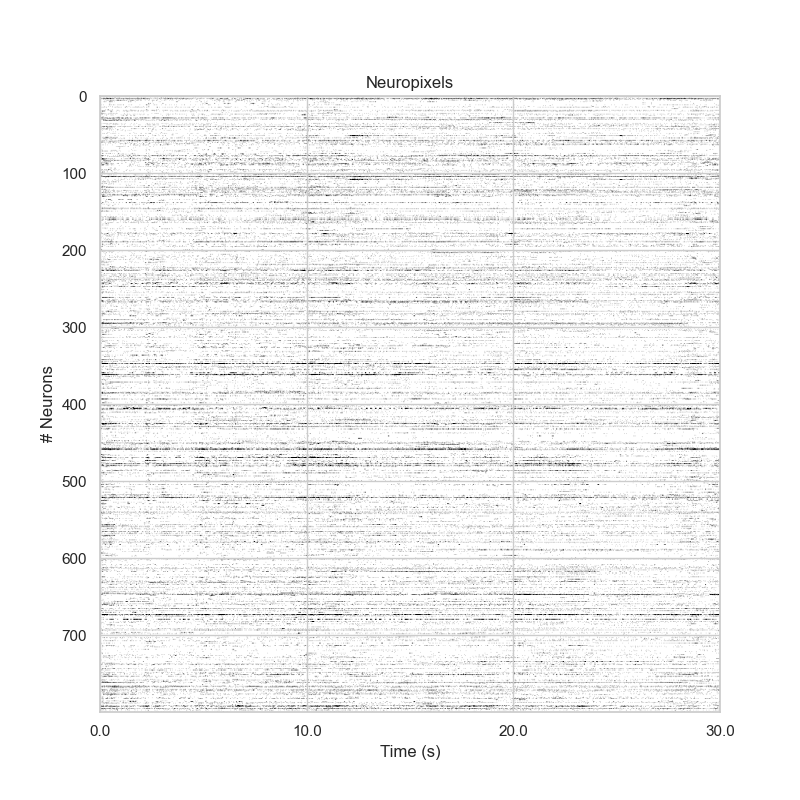
\includegraphics[width=0.6\textwidth]{neuropixels.png}
    \caption{Neural Responses}
    \label{fig:neuropixels}
\end{figure}

We then decided to visualize different dimensionality reductions of the neural responses to see if there is clear clustering. We began with PCA and then moved on to t-SNE. For PCA we used the top $3$ dimensions and each point is colored based on the corresponding frame ID. 

\begin{figure}[H]
    \centering
    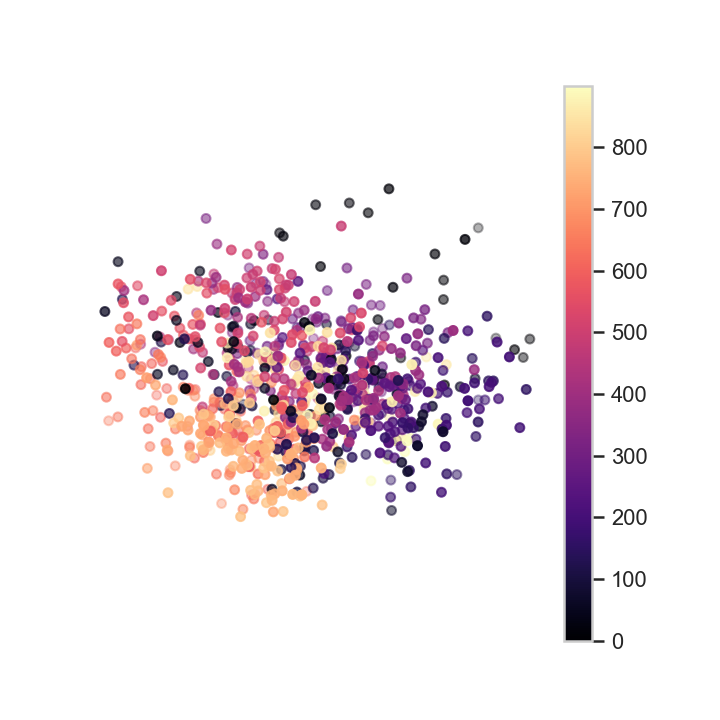
\includegraphics[width=0.5\textwidth]{3d_pca_neuropixels.png}
    \caption{3 dimensional PCA of Neuropixels}
    \label{fig:3d_pca_neuropixels}
\end{figure}

We can see that the PCA plot shows some clustering based on the frame ID but it does not show clear separation between the PCA components for individual frame IDs which would make it difficult to classify. We also plotted the explained variance of the PCA components.

\begin{figure}[H]
    \centering
    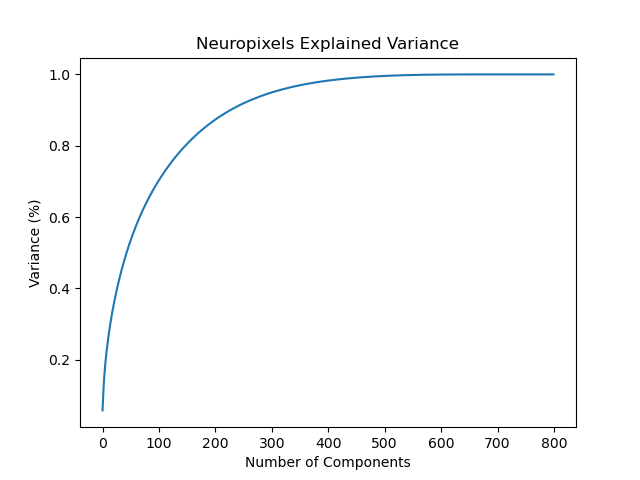
\includegraphics[width=0.5\textwidth]{neuropixels_pca_explained_variance.png}
    \caption{Explained Variance of PCA Components}
    \label{fig:explained_variance_pca}
\end{figure}

From the plot we can see that with around $200$ PCA components we are able to capture $90\%$ of the variance across samples which is only a quarter of the full $800$ neuropixels. We then used t-SNE to visualize the neural responses. We used $2$ dimensions for t-SNE. 

\begin{figure}[H]
    \centering
    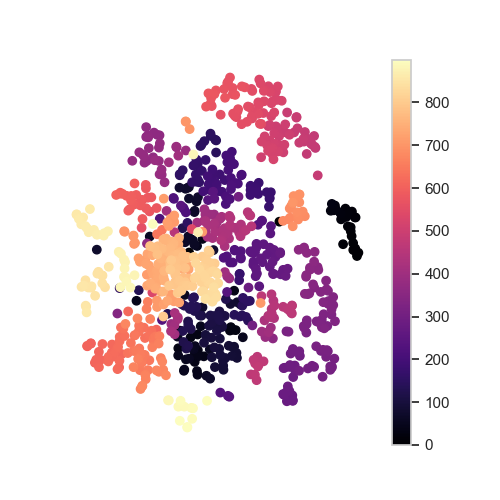
\includegraphics[width=0.5\textwidth]{tsne_neuropixels.png}
    \caption{2 dimensional t-SNE of Neuropixels}
    \label{fig:2d_tsne_neuropixels}
\end{figure}


The t-SNE plot showed clearer separation into clusters based on the frame ID but there was still was not any clear separation between the individual frames. From these plots we can gather that most likely the neural data does not fully encode the information within a frame and most likely only encodes a noisy representation of each frame which is why multiple different frame IDs would be grouped together. This makes sense in the context of the mouse V1 visual cortex because the mouse V1 visual cortex is not a high level visual processing area and is more focused on processing basic visual information.

\subsection{Data Preprocessing}
In order to preprocess the data we first needed to reduce the time dimension for each neuropixel such that the number of stimulus or samples is equal to the number of frames. We did this by taking groups of $4$ bins and then computing the average of the bins in the group. This reduced the number of bins from $3600$ to $900$. So in total we had $9000$ samples rather than $36000$ samples. Next we looked into individual neuropixels. For some neuropixels there activations were $0$ for all frames during a single presentation so we decided to remove those neuropixels. This reduced the number of neuropixels from $800$ to $772$. 

\subsection{Neuropixel Decoding}
We investigated starting from the $772$ neuropixels the decoding $R^2$ score for frame ID using a simple linear regression model. We used $9$ of the stimulus presentations for training and withheld $1$ presentation for test set. We fit a Lasso regression model with alpha the regularization parameter set to $0.08$. 
\begin{figure}[H]
    \centering
    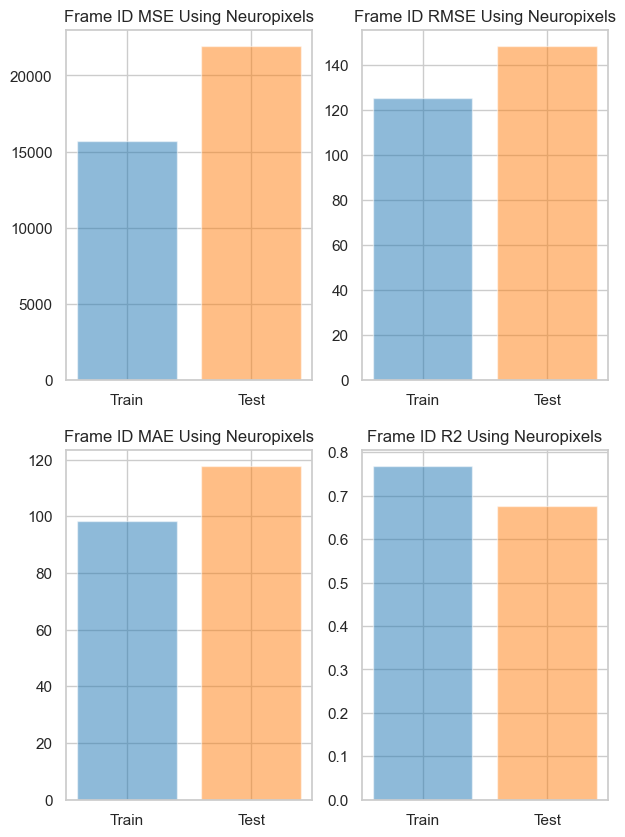
\includegraphics[width=0.5\textwidth]{frame_id_metrics_lasso_.08.png}
    \caption{Lasso Regression Frame ID Decoding}
    \label{fig:lasso_frame_id}
\end{figure}
We can see that there is a high $R^2$ score for the frame ID decoding using the Lasso regression model with the full set of neuropixels used as features. However, the MAE and RMSE are both quite high which could be indicative that the even though the neuropixels are encoding some frame ID information it isn't enough to accurately predict individual frame IDs. Following the results we were interested in seeing how the neuropixel features would perform with logistic regression. We used the same training and test set as before and fit a logistic regression model.

\begin{figure}[H]
    \centering
    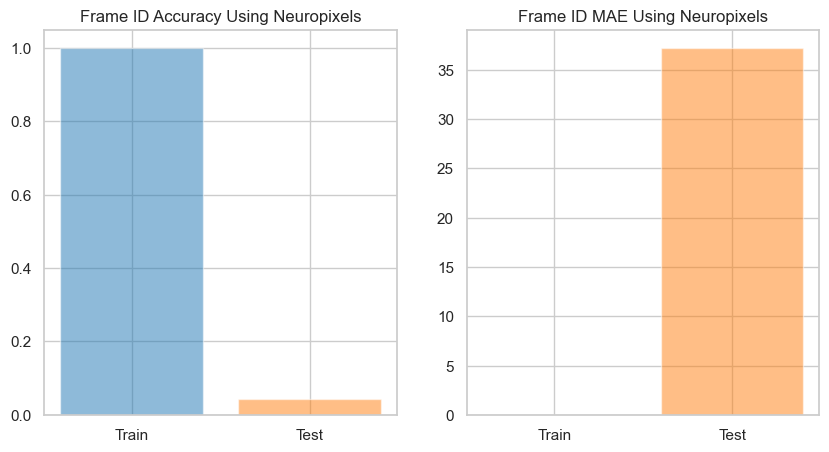
\includegraphics[width=0.7\textwidth]{frame_id_metrics_logistic.png}
    \caption{Train and Test Accuracy and MAE of Logistic Regression Frame ID Decoding}
    \label{fig:neuropixel_logistic_frame_id}
\end{figure}

We can see there is a high overfitting in the model as the training accuracy is at around $1$ but the test accuracy is at around $0.04$. We can also see that the overall MAE or average frame difference is also much higher in the test set compared to the training set. In an attempt to reduce the overfitting we tried the tuning the $C$ or inverse regularization term for logistic regression but the train accuracy was still very high with around the same MAE. Here are the first $10$ decoded frames the logistic regression model predicted on the test set.

\begin{figure}[H]
    \centering
    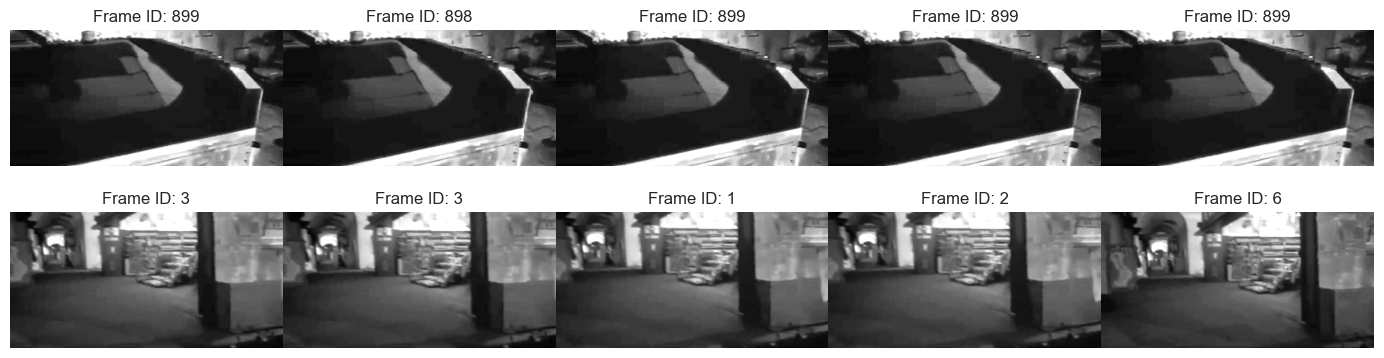
\includegraphics[width=0.8\textwidth]{neuropixel_logistic_reg_video.png}
    \caption{Logistic Regression Decoded Frames}
    \label{fig:neuropixel_logistic_frame_id_decoded}
\end{figure}

We can see that the model predicted the last frame ID for $4$ out of the first $5$ decoded frames and then the following $5$ frames while actually being different frame IDs visually are very similar. This could explain why the decoding accuracy is so poor. The neurons will most likely respond the same way to very similar frames especially in the lower level visual cortex.

\subsection{PCA Decoding}
The neural responses may be very noisy so we were curious if first reducing the dimensionality of the neural responses and then fitting a Lasso or Logistic regression model would improve the frame ID decoding. After fitting a Lasso regression model with $3$ PCA components and an alpha of $0.08$ we got the following results.

\begin{figure}[H]
    \centering
    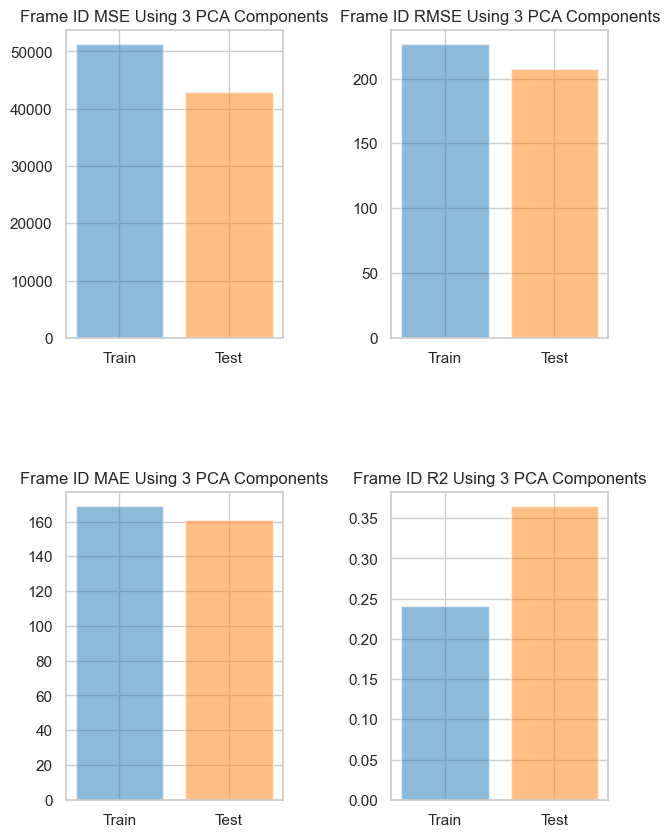
\includegraphics[width=0.5\textwidth]{frame_id_metrics_lasso_using_pca.08.png}
    \caption{Lasso Regression Frame ID Decoding with 3 PCA Components}
    \label{fig:pca_frame_id_lasso}
\end{figure}

We can see that the $R^2$ score is much lower than the full set of neuropixels but the MAE and RMSE are actually very similar to the full set of neuropixels. This could be indicative that the PCA components are actually encoding the same information as the full set of neuropixels. We then fit a logistic regression model with the $3$ PCA components. First we wanted to do a grid search to find the highest performing number of PCA components. Here are the results of the grid search.

\begin{figure}[H]
    \centering
    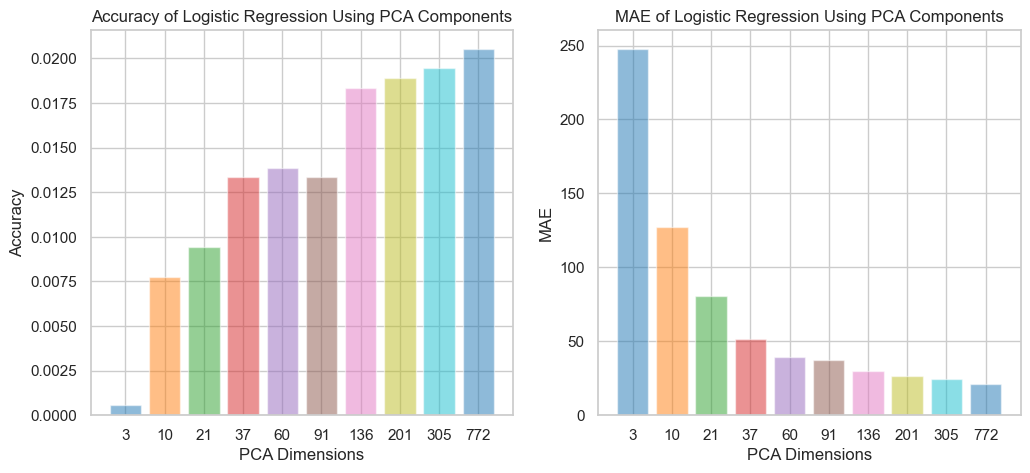
\includegraphics[width=0.7\textwidth]{logistic_pca_accuracy_mae.png}
    \caption{Grid Search for PCA Components in Logistic Regression Frame ID Decoding}
    \label{fig:logistic_pca_accuracy_mae}
\end{figure}

We can see that the highest accuracy is still while using the full $772$ dimensions but we also noticed that even with half as many PCA components the accuracy and MAE are still quite high and similar to the full set of neuropixels. With $305$ dimensions we are able to capture $90\%$ of the variance across samples. Using the $305$ PCA components we fit a logistic regression model and were able to see the following train and test accuracy and MAE.

\begin{figure}[H]
    \centering
    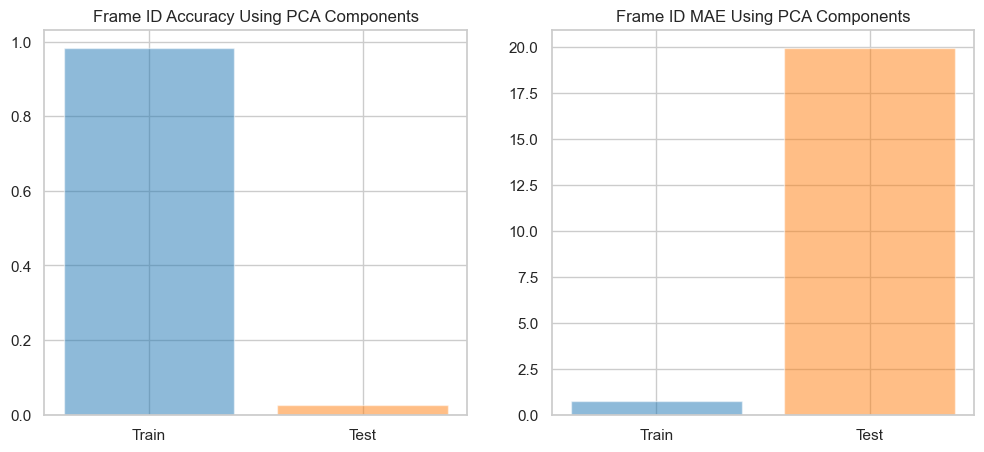
\includegraphics[width=0.7\textwidth]{frame_id_metrics_logistic_C_.4_pca.png}
    \caption{Train and Test Accuracy and MAE of Logistic Regression Frame ID Decoding with PCA Components}
    \label{fig:logistic_pca_frame_id}
\end{figure}

Similar to the full set of neuropixels we can see that there is a high overfitting in the model as the training accuracy is at around $1$ but the test accuracy is at around $.02$ even after applying at $C$ value of $.4$. Notably, while the accuracy is lower than the full set of neuropixels the MAE is actually lower when using the $305$ PCA components. Here are the first $10$ decoded frames the logistic regression model predicted on the test set.

\begin{figure}[H]
    \centering
    \includegraphics[width=0.8\textwidth]{.9_pca_logistic_reg_video.png}
    \caption{Logistic Regression Decoded Frames with .9 Explained Variance PCA Components}
    \label{fig:pca_logistic_frame_id_decoded}
\end{figure}

We can see that the logistic regression model using PCA components is no longer predicting very high frame IDs within the first $10$ frames. The decoded frames however are still not very varied since in this case the frame ID $0$ was actually predicted $4$ times. In addition, similar conclusions can be drawn that the decoded frames despite being different frame IDs are very similar visually.

\subsection{VAE Reconstruction and Decoding}
After exploring some basic classifiers to decode from neural responses to the Frame ID and from PCA components to Frame ID we decided to train a VAE model to reconstruct the neural responses and see if the learned latents could have a better decoding performance for frame ID. We also tested out using different forms of guidance for the VAE model. We tested using no guidance on the latents, a separate head to predict frame ID, and a separate head to predict the PCA components of the dino embeddings. We trained the VAE model for $200$ epochs and used a beta value on the KL divergence of $0.05$ which we found to be the best in terms of validation reconstruction $R^2$ score. We also found that the best model architecture was using $3$ hidden layers in the encoder with LeakyReLU activations in the encoder and $2$ hidden layers in the decoder. For the size of the latent space we used $128$ dimensions the reasoning was mostly to have a valid comparison with the CEBRA latents which also used $128$ dimensions. For the loss function in order to penalize reconstruction we measure the MSE loss between the reconstructed neural responses and the true neural responses in addition to the KL divergence loss. When training the VAE model with guidance on the latents we added an additional loss term that penalized the MSE loss between the predicted dino embeddings and the true dino embeddings or cross-entropy loss between the predicted frame ID and the true frame ID.

\subsubsection{VAE No Guidance}
The following are the results of the VAE model with no guidance on the latents. We measured the model's neural reconstruction $R^2$ score on a train set of $7$ presentations and a validation set of $2$ presentations.

\begin{figure}[H]
    \centering
    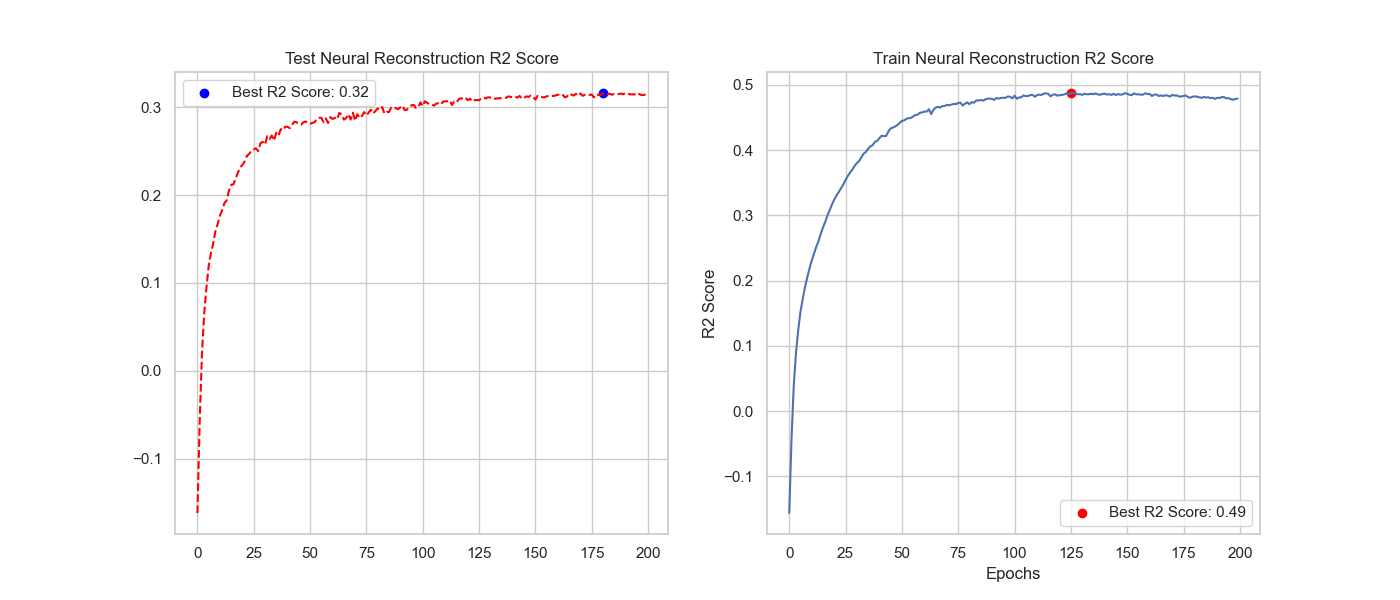
\includegraphics[width=1.0\textwidth]{x_r2_128dim_200_epochs_0.05beta_2_layer.png}
    \caption{VAE No Guidance Reconstruction $R^2$ Score}
    \label{fig:vae_no_guidance}
\end{figure}

We can see from the figure that the model has a decent reconstruction score on the test set for the full set of $772$ neuropixels. The model is able to capture around $30\%$ of the variance in the neural responses. In an effort to improve the reconstruction performance we were curious if taking the neurons with the highest variance across stimulus presentations would reduce noise and improve the $R^2$ score. First we took the top $393$ neurons with the highest variance because using the covariance matrix we were able to measure that with $393$ neurons we could explain approximately $90\%$ of the variance across all stimulus. Specifically, we calculated explained variance by taking the $tr(\Sigma_{features})$ where $\Sigma_{features}$ is the covariance matrix of the top $393$ neurons and dividing it by $tr(\Sigma_{full})$ where $\Sigma_{full}$ is the covariance matrix of the full set of $772$ neurons.

\begin{figure}[H]
    \centering
    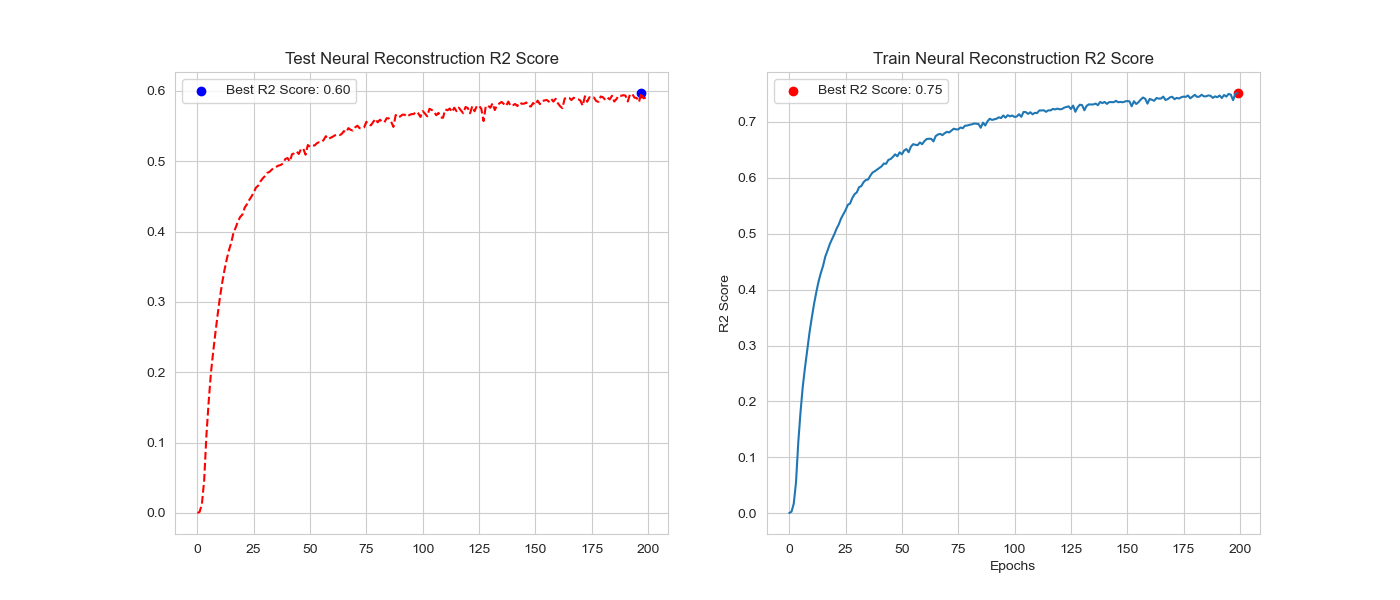
\includegraphics[width=1.0\textwidth]{x_r2_128dim_393_top_var_200_epochs_0.05_beta_2_layer.png}
    \caption{VAE No Guidance Reconstruction $R^2$ Score with Top 393 Neurons}
    \label{fig:vae_no_guidance_top393}
\end{figure}

As expected we see that the $R^2$ score is higher when using the top $393$ neurons compared to the full set of $772$ neurons. Of course the could be attributed to the fact that it is easier for a model to learn a reconstruction when the input has less dimensions but from the PCA exploration of the data the hypothesis is that there are actually many neurons that are not encoding information about the stimulus. We also explored what the reconstruction performance would be if we use the top $503$ neurons which using the same calculations we measured to capture $95\%$ of the variance.

\begin{figure}[H]
    \centering
    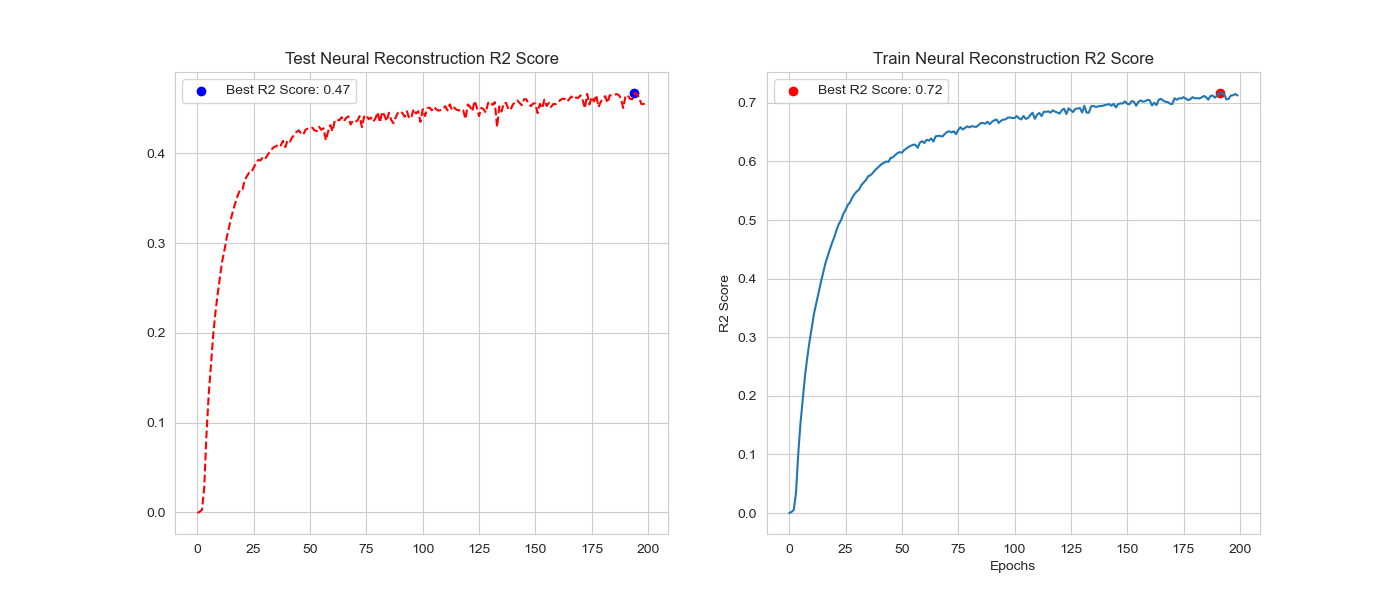
\includegraphics[width=1.0\textwidth]{x_r2_128dim_503_top_var_200_epochs_0.05_beta_2_layer.png}
    \caption{VAE No Guidance Reconstruction $R^2$ Score with Top 503 Neurons}
    \label{fig:vae_no_guidance_top503}
\end{figure}

The test set reconstruction performance using $503$ neurons with the highest variance across stimulus is noticeably lower than with the top $393$ neurons but still higher than the full set of $772$ neurons. With these findings we decided to use the top $503$ neurons for the rest of the VAE models with guidance. 

\subsubsection{VAE Guidance using Dino Embeddings}
The following are the results of the VAE model with guidance on the dino embeddings. We measured the model's neural reconstruction $R^2$ score on a train set of $7$ presentations and a validation set of $2$ presentations. We also measured the model's dino embedding $R^2$ score on the same train and validation set. Initially we used the entire dino embedding as guidance which had $768$ dimensions. During training however we noticed the model's train and validation reconstruction of the embedding stayed in the negatives. We then decided to use PCA to reduce the dino embeddings from $768$ dimensions to $32$ dimensions. The $32$ dimensions were able to capture $90\%$ of the variance across samples. Here are the results of the VAE model with guidance on the PCA of dino embeddings.

\begin{figure}[H]
    \centering
    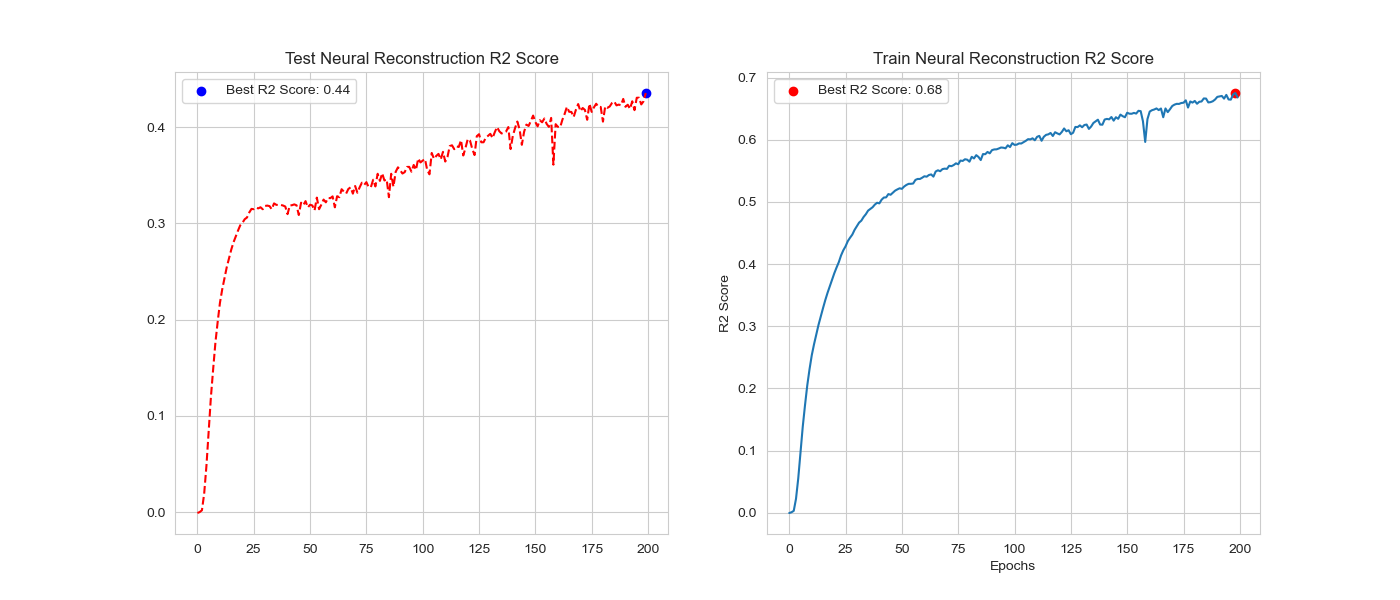
\includegraphics[width=1.0\textwidth]{x_r2_128dim_503_top_var_200_epochs_0.05_beta_2_layer_.9_pca_dino_embed.png}
    \caption{VAE Guidance using Dino Embeddings Neural Reconstruction $R^2$ Score}
    \label{fig:vae_guidance_dino_pca}
\end{figure}

Comparing the reconstruction performance with the no guidance metrics on the top $503$ neurons we can see that the model with guidance on the dino embeddings has a slightly lower reconstruction performance on test with the best $R^2$ score at $.47$ with no guidance and $.44$ with guidance. Next we wanted to see if the model was able to reconstruct the dino embeddings well.

\begin{figure}[H]
    \centering
    \includegraphics[width=.9\textwidth]{.9_pca_dino_embed_r2_128dim_503_top_var_200_epochs_0.05_beta_2_layer.png}
    \caption{VAE Guidance using Dino Embeddings Dino Embedding $R^2$ Score}
    \label{fig:vae_guidance_dino_pca_dino_embed_r2}
\end{figure}

Above we plotted the dino embedding $R^2$ score for the validation and training sets starting at epoch $50$ in the training process. The reason is because the dino embedding $R^2$ score was negative at the beginning of training. We can see that the model was able to learn to capture some of the variance between dino embeddings with the best $R^2$ score at $.19$ on the validation set and $.23$ on the training set.

\subsubsection{VAE Guidance using Frame ID}
We also attempted to directly use the frame ID as guidance for the VAE model. We mapped from the $128$ dimensions of the latent space to a $900$ dimensional vector which was used in the cross-entropy loss. Below are the results of the VAE model with guidance using the frame ID.

\begin{figure}[H]
    \centering
    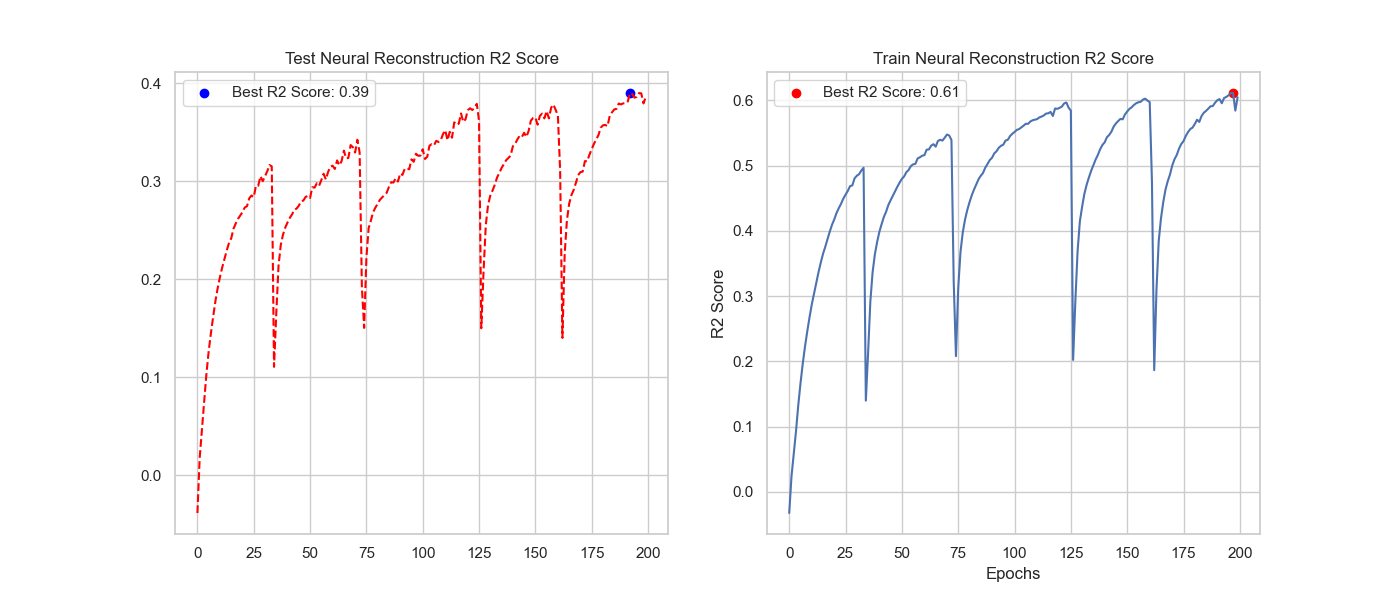
\includegraphics[width=1.0\textwidth]{x_r2_128dim_503_top_var_200_epochs_0.05_beta_2_layer_frame_id_guidance.png}
    \caption{VAE Guidance using Frame ID Neural Reconstruction $R^2$ Score}
    \label{fig:vae_guidance_frame_id}
\end{figure}

The model using frame ID shows significantly lower $R^2$ scores for neural reconstruction compared to the model with guidance on the dino embeddings and when using no guidance. In addition, we can see that during the training process there are sharp drops in the training and test $R^2$ scores which we did not see in the other models. 

\end{document}
